\documentclass[/home/nkappler/Research/Dissertation/
 dissertation.tex]{subfiles}

\begin{document}

\chapter{Inverse Niche Models}

\begin{bibunit}

\begin{abstract} 

    The niche model \cite{Williams2000} has been remarkably successful at
    predicting the structure of trophic food webs. A wide range of network
    properties of food webs are well predicted with only two inputs to the
    model. However, there are valid concerns about its ability to predict the
    structure of more complex food webs involving novel consumer strategies not
    based on the assumed body size hierarchy \cite{Williams2011}. We expand the
    inverse niche model \cite{Warren2010} and show that matching connectances
    of the free liver - free liver, parasite - free liver, free liver -
    parasite, and parasite - parasite subwebs individually results in an
    improved fit over a null model with randomly chosen parasites.  

\end{abstract}

\newpage

\section{Introduction}

Existing models of food web structure have proven able to capture key
properties of ecological networks \cite{Williams2000, Allesina2008,
Williams2010, Williams2008b}. A potential drawback of these models is that they
were designed and verified almost exclusively on predator-prey food webs. Thus,
modern webs that incorporate many species and diverse types of interactions
among species \cite{Kefi2016, Hechinger2011a, Thieltges2011, Zander2011,
Mouritsen2011} may not be well modeled by these food web models. A recent study
verified that food webs incorporating parasites were poorly modeled by the
probabilistic niche model but that the lack of fit was consistent with a
generic loss of performance on larger and more complex webs \cite{Dunne2013}. 

A key feature in many of the food web models is the existence of a ``niche
axis'' in which species can be ordered. A species's location in this axis
determines who it eats and by whom it is eaten. The niche axis has been found to be
highly correlated with body size; a probabilistic niche model inferring niche
values from food web data showed that body sizes and niche values estimated via
maximum likelihood were highly correlated with $r=0.883$ in a marine food web
\cite{Williams2010}. Note, however, that the same authors found substantial
variation in the structure of the niche axis in a large set of different
empirical food webs \cite{Williams2011}. Some larger webs required two separate
niche axes (that is, two separate trait hierarchies) to be accurately captured
by a niche model. To what extent can a single trait axis accurately and
simultaneously model disparate interactions such as those between parasites and
hosts and free living hosts and their prey?

\cite{Warren2010} designed the inverse niche model as a way to more accurately
capture the unique roles of parasites in food webs while still using a single
trait axis. They found that relaxing certain assumptions of the niche model and
imposing a reversed generality hierarchy on parasites resulted in a
significantly better fit over a niche model with parasites chosen randomly
among the consumers. We extend and clarify several aspects of the inverse niche
model and compare its performance on 6 species rich and highly resolved food
webs. We supplement this earlier work on the inverse niche model by clarifying
and expanding its definition and testing its performance on a set of six highly
resolved food webs containing parasites, including an updated version of the
empirical web originally studied in \cite{Warren2010}.

%Assessing the fidelity of food web models is challenging.  Previous studies
%have computed a laundry list of ecological properties for many simulated webs
%and compared the resulting distribution to the properties on one or several
%known webs \cite{x,y,z}. The theoretical model that has the most empirical
%properties within some normalized error limit is declared the most faithful. This
%relatively simple and straightforward procedure has the benefit of transparency
%but is somewhat lacking in its rigor; for example, it is very difficult to
%construct a $P$-value. 
%
%When counting the number of properties that a food web model accurately predicts,
%the acceptable limits are usually taken to be the middle 95\% of the empirical data
%(lower or upper 95\% as appropriate for skewed properties). This produces a
%reasonable measure of model fidelity if we consider the vector of observed
%properties to be generated by a non-random process. This assumption is somewhat
%peculiar as much of the usefulness of statistics in the natural sciences comes
%from treating observations as random outcomes. \fxwarning{Definitely revisit
%this! I don't think this is an accurate representation!} As a baseline, we use
%the above method of assessing fideltiy, and explore several other procedures;
%in our alternative procedures, we generally consider the empirical webs to be
%stochastically generated observations of the space of empirical food webs.
%
%As mentioned above, the standard procedure of counting the number of properties
%within some error bounds is appropriate if the empirical data are considered 
%constants. We instead model the empirical properties as samples from the space
%of empirical food webs with the same species diversity and link complexity.
%Thus, in what follows we are generally considering $\mathbf{x}$, the vector of
%observed properties of an empirical web, to be an observation from some unknown
%distribution and we are assessing the ability of the food web model to
%accurately capture that value.

\section{Methods}

\subsection{Niche Model} 

The niche model was originally proposed in \cite{Williams2000} and makes the
following four assertions about how trophic interactions are formed between
species.

\begin{enumerate}
    \item The abstract space of species niches (the infamous ``$n$-dimensional
        hyperspace'') can be mapped onto the interval $(0,1)$,
        hereafter, the ``niche axis.''
    \item The diet of a species consists of an interval within the niche
        axis, hereafter, the species's ``feeding range''.
    \item The width of a  species's feeding range is proportional to the
        species's value on the niche axis, AND
    \item The center of a species's feeding range is at or below the species's
        value on the niche axis.
\end{enumerate}

Thus, the niche model proposes a semi-hierarchical ordering of species with
contiguous diets. The niche model generates candidate food webs given a species
richness and web connectance via the following algorithm, which requires just
species richness, $S$ and food web connectance, $C$ as its inputs:

\begin{enumerate}
    \item For each species, pick a niche value, $n_i$, from a $U(0,1)$ distribution.
    \item For each species, pick a diet proportionality constant, $y_i$ from a
        $\text{Beta}(1,\beta)$ distribution (see below for a discussion of
        $\beta$). The width of species $i$'s feeding range is $r_i = n_iy_i$.
    \item Pick a diet center, $c_i$ for each species uniformly at random from
        the niche axis such that the diet center is (a) less than the species's
        niche value, and (b) the diet is entirely contained within the niche
        axis.
    \item Species $i$ eats species $j$ if $j$'s niche value falls within the
        feeding range of $i$.
\end{enumerate}

Candidate webs are rejected if they are not weakly connected or if their
connectances are not within 3\% of the target connectance. The target
connectance is matched by choosing an appropriate $\beta$ parameter for the
beta distribution. The $\beta$ parameter is chosen so that
$\mathbb{E}[n_iy_i]=C$. Thus, we require that $\mathbb{E}[y_i]=2C$ and it
immediately follows that we must have $\beta = \frac{1-2C}{2C}$; this single
parameter accounts for the patterns of complexity seen in webs at a given
species richness. Figure \ref{fig:nicheModel} diagrams the process. The result
of this algorithm is a network structure. Numerous studies have demonstrated
the efficacy of this model and its variants
\cite{Williams2000,Allesina2008,Williams2008b}.

As a null model, We select species to be parasites in the niche model uniformly
at random from the consumers in a niche model web. The empirical data has
parasitic nodes exclusively parasitizing nodes with trophic level greater than
one; however, niche model webs at the necessary size and complexity generally
do not have enough carnivores to support the necessary number of parasites. We
will compare this model of food webs with parasites to several variants of the
inverse niche model proposed in \cite{Warren2010}.

%\begin{itemize}
%    \item A species's trophic niche can be decomposed into two interrelated
%        sub-niches: a resource niche and a consumer niche.
%    \item There exists a continuous mapping from the abstract resource niche
%        onto the interval $(0,1)$. The value that a species's resource niche
%        is mapped to is called the species's `niche value.'
%    \item There exists a continuous mapping from the abstract consumer niche
%        onto the set of interval subsets of $(0,1)$. The resulting interv
%    \item 
%    \item The resource niche and the consumer niche are related to each other
%        such that a consumers prey tend to have lower resource niches than the
%        consumer, AND
%    \item species whose resource niches are mapped to larger numbers in $(0,1)$
%        tend to have wider consumer niches.
%\end{itemize}

%Species with similar niche values tend to have similar sets of consumers; 
%species with similar prey sets do not necessarily have similar niche values

%Imposition of uniformity on all individuals in a species?

\begin{figure}
    \centering
    \begin{tikzpicture}
        \draw (0,0)--(10,0)
        node[anchor = west] {$n$};
        \draw (0,.2)--(0,-.2)
        node[anchor = north] {$0$};
        \draw (10,.2)--(10,-.2)
        node[anchor = north] {$1$};
        %Predator
        \fill (7,0) circle (.07) 
        node[anchor = north]  {$n_j$};
        %Predator Diet
        \draw (7,0)--(7,.75)--(2,.75)--(2,.5);
        \draw (.3,0) -- (.3,.5) -- (3.7,.5) -- (3.7,0);
        \draw[dashed] (2,.5) -- (2,0) 
        node[anchor = south east] {$c_j$};
        \draw[<->] (.3,-.5) -- (3.7,-.5)
        node[fill=white,pos = 0.5] {$r_j$}; 
        \draw[dashed] (.3,0)--(.3,-.55);
        \draw[dashed] (3.7,0)--(3.7,-.55);
        %Prey
        \fill (3,0) circle (.07) 
        node[anchor = north west]  {$n_i$};
        \draw(4.2,-1.2) circle (.3)
        node {$i$};
        \draw[->] (4.5,-1.2) -- (5.5,-1.2);
        \draw(5.8,-1.2) circle (.3)
        node {$j$};
    \end{tikzpicture}
    \caption[Niche model diagram]{This figure demonstrates how feeding relationships are determined
    in the Niche Model.\label{fig:nicheModel}}
\end{figure}


\subsection{Inverse Niche Models}
The inverse niche model was originally proposed in \cite{Warren2010}. We first
outline the structure of the inverse niche model and then propose three
refinements based on the proportionality constant between a species's niche value
and its feeding range.

\subsubsection{Original Inverse Niche Model} 

The original inverse niche model was shown to better predict many observed
ecological properties of an earlier version of the Carpinteria Salt Marsh food
web. This was achieved by ``inverting'' both the feeding hierarchy and the
generality hierarchy.  Parasites in the inverse niche model have diet centers
above their niche value (inverted feeding hierarchy) and diet widths
proportional to $1-n_i$ (inverted generality hierarchy). The original inverse
niche model also altered the distribution of proportionality constants for
parasites so that the connectance of parasite-host interactions was accurately
captured. Figure \ref{fig:invNicheModel} diagrams the inverse niche model. We
modify this basic procedure by centering the diets of parasites on the niche
value of a free-living species; that is, the feeding range of a parasite is
always centered on a free-liver. If this resulted in any portion of the diet
lying outside the niche axis, we shifted the feeding range up or down so that
it was entirely contained in the niche axis. This was done to ensure that
parasites always have a host and to minimize the number of rejected webs.


\begin{figure}
  \centering
    \begin{tikzpicture}
        \draw (0,0)--(10,0)
        node[anchor = west] {$n$};
        \draw (0,.2)--(0,-.2)
        node[anchor = north] {$0$};
        \draw (10,.2)--(10,-.2)
        node[anchor = north] {$1$};
        %Predator
        \fill (7,0) circle (.07) 
        node[anchor = south west]  {$n_j$};
        %Parasite 
        \fill (1,0) circle (.07) 
        node[anchor = south]  {$n_p$};
        %Predator Diet
        \draw (7,0)--(7,.75)--(2.8,.75)--(2.8,.5);
        \draw (1.3,0) -- (1.3,.5) -- (4.3,.5) -- (4.3,0);
        \draw[dashed] (2.8,.5) -- (2.8,0) 
        node[anchor = north] {$c_j$};
        \draw[<->] (1.3,1.2) -- (4.3,1.2)
        node[fill=white,pos = 0.5] {$r_j$}; 
        \draw[dashed] (1.3,0)--(1.3,1.25);
        \draw[dashed] (4.3,0)--(4.3,1.25);
        %Prey
        \fill (3,0) circle (.07) 
        node[anchor = south west]  {$n_i$};
        \draw(3.4,-2) circle (.3)
        node {$i$};
        \draw[->] (3.7,-2) -- (4.7,-2);
        \draw(5,-2) circle (.3)
        node {$j$};
        \draw[->] (5.3,-2) -- (6.3,-2);
        \draw (6.6,-2) circle (.3) node {$p$};
        \draw (1,0) -- (1,-0.75) -- (7,-0.75) -- (7,-0.5);
        \draw (5.5,0) -- (5.5,-0.5) -- (8.5,-0.5) -- (8.5,0);
        \draw[<->] (5.5,-1.2) -- (8.5,-1.2)
        node[fill=white,pos = 0.5] {$r_p$}; 
        \draw[dashed] (5.5,0)--(5.5,-1.25);
        \draw[dashed] (8.5,0)--(8.5,-1.25);
        ]
    \end{tikzpicture}
  \caption[Inverse niche model diagram]{This figure demonstrates how feeding relationships are determined in
  the inverse niche model.\label{fig:invNicheModel}}
\end{figure}

We could not determine from \cite{Warren2010} whether or not links between
parasites or links from parasites to free-livers were allowed in their model. To
be clear, we have allowed them, ensuring an accurate comparison to
observed data, as all of these links were present in the empirical data (table
\ref{tab:allCs}).

\begin{table}
        \centering
        \begin{tabular}{r l l l l l}
            \toprule
            Full Name&  $C$ &$C_{f\!f}$ &$C_{f\!p}$  &$C_{p\!f}$   &$C_{pp}$\\
            \midrule
            Bahia Falsa San Quintin&0.083&0.098&0.092&0.075&0.036\\
            Carpinteria Salt Marsh&0.084&0.090&0.121&0.050&0.053\\
            Estero de Punta Banda&0.079&0.072&0.139&0.052&0.064\\
            Flensburg Fjord&0.090&0.090&0.152&0.040&0.069\\
            Otago Harbor&0.077&0.082&0.079&0.048&0.066\\
            Sylt Tidal Basin&0.071&0.112&0.081&0.023&0.021\\
            \bottomrule
        \end{tabular}
    \caption[Subweb connectances]{This table reports the connectances of the four subwebs defined by
        free liver - free liver $(C_{f\!f})$, free liver - parasite $(C_{f\!p})$,
        parasite - free liver $C_{p\!f}$, and parasite - parasite $C_{pp}$
        interactions in all 6 empirical food
webs.\label{tab:allCs}}
\end{table}

\subsubsection{Updated Inverse Niche Models}

We test three different versions of the inverse niche model, each matching
different connectances in the observed food web. In the first version, to more
accurately compare the inverse structure to the null model, we don't adjust the
proportionality constant of parasite species to match the observed parasitic
connectance. Instead, we choose the parameter so that parasites and free-living
consumers both have the same expected generality. This was done by choosing a
beta constant for parasites as $\beta_p = \frac{1-2C'}{2C'}$ ($\beta_f =
\frac{1-2C}{2C}$ is the parameter for free-livers), where $C'$ is an adjusted
connectance accounting for the fact that parasites are consumers by definition.
We compute the adjusted connectance as follows, in which $S_f$ is the richness
of free-living species:

\begin{equation}
    C' = \frac{CS^2 - CS_fS -S_p}{(S_f-1)Sp}\label{eq:Cp0}
\end{equation}

The idea behind this correction is that $S_p$ of the links pointing toward
parasites (one per parasite) are a given; thus the random number of links
defined by the feeding range needs to be smaller to match the target
connectance. We consider this model to be a more even comparison to the null
model than was achieved in \cite{Warren2010}.

The second inverse niche model model is identical to the original inverse niche
model except for those differences mentioned above. In this model, we choose
$\beta_p$ to match the parasite connectance, which we define as follows:

\begin{equation}
    C_{p} = \frac{L_{ p}}{SS_p}\label{eq:Cf}
\end{equation}

In which $L_{p}$ is the number of links pointing towards a parasite. In
this model, $\beta_p$ is calculated as

\begin{equation}
    \beta = \frac{1-2C'_{ p}}{2C'_{ p}}\label{eq:beta2}
\end{equation}

In which we define the adjusted parasite connectance, $C'_{ p}$, as

\begin{equation}
    C'_{ p}=\frac{CS^2 - C_{ f}S_pS_f - S_p}{(S-1)S_p}\label{eq:CpAdj}
\end{equation}

Note that $C_{ f}$  is the free-liver connectance defined in the same way as
$C_{ p}$; the beta parameter for free livers is $\beta_f=\frac{1-2C_f}{2C_f}$.
This model has four independent inputs: $S$, $S_p$, $C$, and $C_f$. We use
$C_f$ instead of $C_p$ out of convenience. Given $C$, $S$, $S_p$, and $C_f$ one
can calculate $C_p$ exactly.

The final model we considered matches all four subweb connectances described in
table \ref{tab:allCs}. This required defining four different $\beta$
parameters; the formula for each is given in equations
\ref{eq:allBetasff}-\ref{eq:allBetaspp}.

\begin{align}
    \beta_{f\!f} &= \frac{1-2C_{f\!f}}{2C_{f\!f}}\label{eq:allBetasff}\\
    \beta_{f\!p} &= \frac{1-2C'_{f\!p}}{2C'_{f\!p}}\\
    \beta_{p\!f} &= \frac{1-2C_{p\!f}}{2C_{p\!f}}\\
    \beta_{pp} &= \frac{1-2C_{pp}}{2C_{pp}}\label{eq:allBetaspp}
\end{align}

Where once again we correct the connectance in the formula for $\beta_{f\!p}$ as
follows:

\begin{equation}
    C'_{f\!p} = \frac{CS^2 - C^{ }_{f\!f}S_{f\!f}^2 -C_{p\!f}S_pS_f
        -C^{ }_{pp}S_p^2 -
    S_p}{(S_f-1)S_p}\label{eq:CfpAdj}
\end{equation}

The four beta parameters were used to define two different feeding ranges for
each species. One of these feeding ranges determines the consumption of
parasites; the other determines the consumption of free livers. The two feeding
ranges share a diet center. 

\begin{table}
    \begin{tabular}{r l l l}
        \toprule
        \multicolumn{2}{l}{Parasite Model}  & Inputs \\
        \midrule
        1. & Randomly Chosen from Niche model&$S$, $S_p$, $C$\\
        2. &Inverse NM, widths match $C$.& $S$, $S_p$,
        $C$\\
        3. &Inverse NM, widths match $C_p$, $C_f$& $S$, $S_p$,
        $C$, $C_f$\\
        4. &Inverse NM, widths match subweb connectances& $S$, $S_p$,
        $C$, $C_{f\!f}$, $C_{f\!p}$, $C_{p\!f}$\\
        \bottomrule
    \end{tabular}   
    \caption[Summary of food web models tested]{This table summarizes the inputs to each of the four models. All
    models had the same rejection criteria for candidate food webs; the
    networks  must be weakly connected, all species must be connected to basal
    species, and overall connectance must be within 3\% of the target overall
    connectance. We do not check that individual subweb connectances are
    individually matched.\label{tab:invNMSummary}}
\end{table}


\subsection{Assessing Models}

In this section we describe the laundry list of ecological network properties
that were assembled and then outline several alternative approaches to the
problem of model assessment. 

\subsubsection{Building a Laundry List}

We attempted to construct a comprehensive list of network properties to assess
as many features of the food web models as possible. Many of the properties
below are found in other studies of food webs; some of these common properties
are redefined or changed outright. In this section we explain the rationale for
any changes or additions to the standard list of roughly 15 properties.

In addition to calculating properties with respect to the entire food web, we
also calculate properties with respect to the communities of free livers and of
parasites. There is significant overlap between the properties calculated and
we note which properties are calculated on the free liver and parasite
communities in table \ref{tab:assProps}.

We use the classic definition of omnivory (an omnivore is a consumer that
consumes both basal and consumer species) and not the trophic definition (an
omnivore is a species with resources at two different trophic levels). This
change was made because we wanted a metric that distinguished, for example, a
species with prey at trophic levels 1 and 2 from a species with prey at trophic
levels 2 and 2.5.

The correlation between generality and vulnerability was used instead of the
standard deviation of the total number of links since it is a more direct
representation of the new information present in the standard deviation of
links. 

We also calculate the average ecological betweenness measure for all species
and both communities. We calculate in each community the mean vulnerability of
resources, mean generality of consumers, and mean FlowRank measures. Since the
FlowRank is normalized to have its entries positive and sum to 1, we calculate
the standard deviation of FlowRank of all species in the web.

\begin{table}
    \begin{tabular}{l p{4in}}
        \toprule
        Property & Comments\\
        \midrule
        \multicolumn{2}{l}{Global and Comm. Props.}\\\cmidrule{1-1}
        TOP,INT,BAS&The fraction of top, intermediate, and basal species in the
        web, respectively.\\
        HERB,CARN&The fractions of herbivores and carnivores,respectively.\\
        OMN&The fraction of species that consume both a basal and a non-basal
        species. The set $\{$TOP,INT,BAS,HERB,CARN,OMN$\}$ has only
        four degrees of freedom.\\
        CANN&The fraction of cannibals in the food web.\\
        $\rho_{gv}$&The correlation between generality and vulnerability.\\
        $\sigma_{g}$&The standard deviation of generality.\\
        $\sigma_{v}$&The standard deviation of vulnerability.\\
        $TL$&The mean prey-averaged trophic level.\\
        FlowRankSD&The standard deviation of the FlowRank metric.\\
        PATH&The average link distance of every species to every other.\\
        Loop&The fraction of species involved in a loop.\\
        EcoBtwn&The mean Ecological Betweenness over all species.\\
        $\gamma^{c}$, $\gamma^{r}$, $\gamma^{rc}$, and $\gamma^{cr}$.& The
        clustering coefficients discussed in chapter 2.\\
        MaxSim&The average of the maximum similarity of each species to all
        other species.\\
        \midrule
        Community Properties\\\cmidrule{1-1}
        $\overline{v}$,$\overline{g}$&Mean vulnerability and mean generality.\\
        FlowRank&As described in chapter 2.\\
        $C_{EB}$&Ecological Betweenness as described in chapter
        2.\\
        $v_r$ and $g_c$&Mean vulnerability of resources and mean generality of
        consumers.\\\bottomrule  
    \end{tabular}
    \caption[Laundry list of network properties]{This table reports the properties used assess the
    ability of the food web models to accurately capture empirical food web
    structure.
    \label{tab:assProps}}
\end{table}

\subsubsection{Likelihood Ratios}

As mentioned above, the standard assessment of fidelity is based solely on
counting the number of properties that are likely to have been accurately
modeled in a food web. We supplement these numbers by providing likelihood
ratios relative to the null model for each model of food web structure. To do
this, we assume that the number $x$ of $n$ properties within a range of
percentiles of width $p$ (expressed as a proportion) follows a
$\text{Bin}(n,p)$ distribution. We calculate the logarithm of the likelihood
ratio of each inverse model relative to the null model. Hence, for each inverse
niche model, we define the log-likelihood ratio as 

\begin{equation}
    L =
    \log\left(\frac{\binom{n}{k}p^k(1-p)^{n-k}}{\binom{n}{k_0}p^{k_0}(1-p)^{n-k_0}}\right)\label{eq:LL1}
\end{equation}

Where $k$ is the number of properties correctly predicted by the inverse niche
model under consideration, $k_0$ is the number of properties correctly
predicted by the null model, and $n$ is the total number of properties
considered.

Equation \ref{eq:LL1} makes the strong assumption of independence of the
properties. This is demonstrably incorrect since, for example, the TOP,
INT, and BAS properties sum to 1. Beyond such simple relationships, several
properties in each ensemble can be very well modeled by linear regression
models based on the other properties, with $R^2$ values exceeding 0.9. This is
the well-known problem of multicollinearity, often arising in multivariable
linear regression. The issue in this setting is different from that in linear
regression since high multicollinearity of the data can cause significant
dependence among the properties that are able to be accurately predicted.

As an illustration of the problem, consider the following situation.
Suppose pigs are judged at a county fair and awarded ribbons according to the
following criteria: (1) weight, (2) volume, and (3) mass.
Clearly, a pig that wins a blue ribbon in the first category is likely to win a
blue ribbon in the remaining two. These three categories are all ways to
measure ``bigness.'' If instead the categories are (1) weight, (2) tail curl,
and (3) skin complexion, a single pig is much less likely to win all three
categories; any pig that does is truly remarkable. Three independent  
properties of pigginess are measured in the second set of criteria.

On the other hand, when grading pigs by the first criteria, we can clearly
distinguish truly pathological pigs. The county fair example implicitly assumes
we are measuring living pigs but those three categories would be good at
distinguishing pigs at a given weight made of metal or foam. Thus, we should
also be aware of properties that are correlated by sampling biases (i.e. only
comparing living pigs) and properties that are correlated by necessity (the
mass and weight of a pig cannot help but be perfectly correlated). 

There are many approaches to this problem; we chose to address it by computing
the principal components of the ensemble data. Working in the transformed
coordinate frame allowed us to calculate percentiles of the empirical webs in
independent linear combinations of the original data. The counts in this case
are much better modeled by binomial random variables and the likelihood ratios
are better representations of the way that empirical webs fit into the variance
patterns of the ensemble data. Note that in our analysis we dropped any
linearly dependent columns in the data. Often, the variables dropped were
simply INT and OMN, though some ensembles at some aggregation levels had
degenerate properties that were equal to 0 for every web in the ensemble; such
properties were also dropped. 

To summarize, for each food web model, we compute the number of empirical
properties within each error range and compute likelihood ratios for each
inverse niche model. This is done using both the raw data and the principal
components. These values are reported for the set of global level properties
and the set of community level properties for both free livers and parasites.

\subsubsection{Food Web Aggregation}

We consider the above analyses in detail on the original webs and also provide
a summary of the performance on each web at four minimum cluster distances in
the sequence of aggregated food webs from chapter 2. We report the likelihood
ratio and the number of missed properties as calculated on the raw data and the
principal components.
 
\subsection{Summary}

We generated 1000 webs according to the 4 models above for each of the 6
empirical food webs. Thus, we generate 4000 model webs for each of the
aggregated empirical webs with minimum cluster distances of 0, 0.05, 0.1, 0.2,
and 0.4. For a graphical representation of the results on the original food
webs, we calculate the model error (ME) for a given property, empirical web,
and food web model as the logit-transformed percentile of each empirical
property within the model ensemble. If a property was skewed (skewness $>$ 0.5)
we calculated instead the appropriately centered logarithm of the percentile.
These are plotted in figures \ref{fig:NMPropsRaw} and \ref{fig:NMPropsPCA} to
give a graphical overview of the performance of each food web model.

\section{Results}

\subsection{Raw Properties}

The food web models in general failed to capture the majority of the properties
of the empirical webs and many of the properties were completely outside the
bounds of the properties observed in the web ensembles. Figure
\ref{fig:NMPropsRaw} gives a graphical representation of the transformed
percentiles of each property for each web and each model. The inverse niche
model that matches all subweb connectances accurately predicts significantly
more of the global properties than the other 3 food web models. Its performance
on the free liver properties is not significantly different from the other
models. The model that matches subwebs also predicts more of the parasite
properties, though it still matches less than 40\% of them. This represents a
marked improvement of 30-40\% over the other 3 models.

More properties tend to be under-predicted than over-predicted by the food web
models across all the webs and food web models; the subweb model connectances
had the fewest properties over-predicted for all three sets of properties
considered. 

\begin{sidewaysfigure}
    \centering
    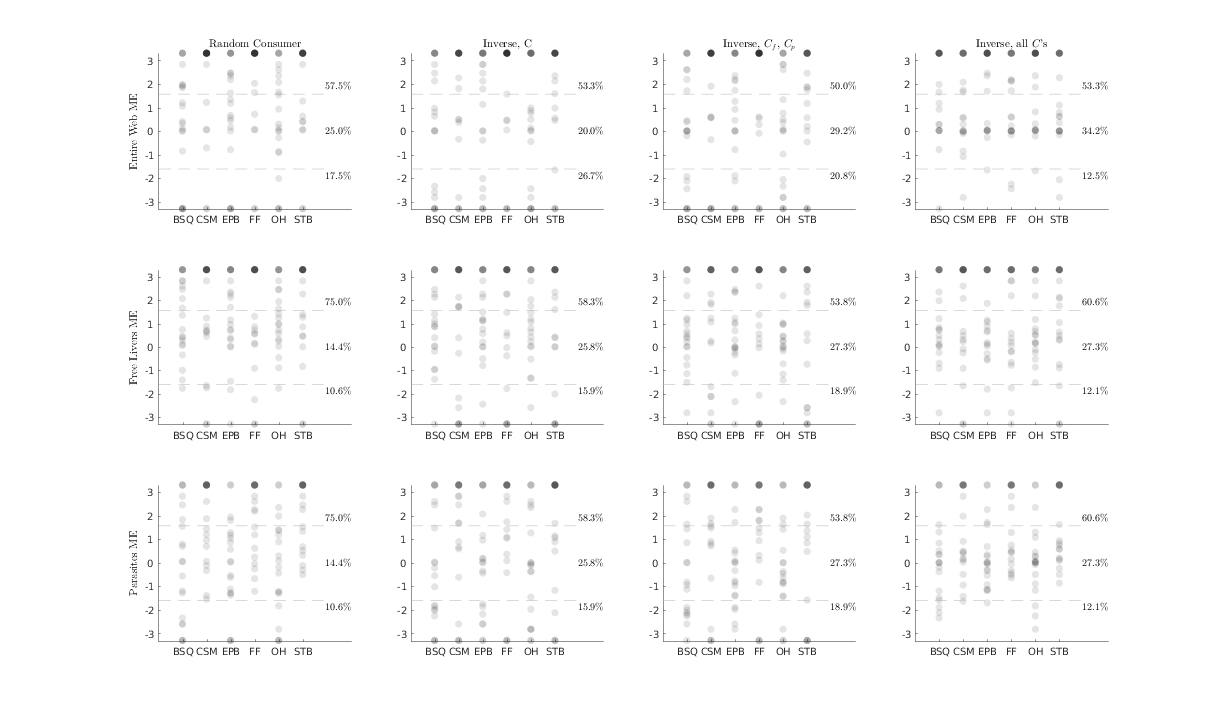
\includegraphics[width=\linewidth]{\DissertationDir/Chapter3/figures/Properties-Raw.png}
    \caption[Niche model properties predicted]{This figure shows logit transformed percentiles of the raw
        properties of the empirical webs within the model ensemble. The line of
        points at $\approx\pm$3.3 denote empirical properties completely
        outside the bounds of observed values in the web ensemble; the shading
        of these dots indicate the relative number of properties outside the
       range of the ensemble data.
    \label{fig:NMPropsRaw}}
 \end{sidewaysfigure}

The performance of the subweb model relative to the other models when
predicting properties of the entire web (figure \ref{fig:ErrorsAggRaw},
top row) does not qualitatively change as aggregation is increased. The
likelihood ratios demonstrate that the performance of the inverse niche models
generally decline relative to the null model as trophic resolution is
decreased. At a minimum cluster distance of 0.4, the subweb model still
outperforms the null model, though by a smaller margin than at lower cluster
distances. The other inverse niche models show only marginal improvements over
the null model at minimum cluster distances less than 0.2 and perform worse
than the null model at minimum cluster distances of 0.4.

When predicting the properties of the parasitic community (figure
\ref{fig:ErrorsAggRaw}, bottom row), the subweb model was again consistently
better than the other three food web models. This performance tended to
increase, both in the number of properties predicted per web, and relative to
the null model as trophic resolution was decreased. The null model generally
performed as well as the connectance and generality models.

All models had essentially the same performance on free liver properties
(figure \ref{fig:ErrorsAggRaw}, middle row) at minimum clustering distances of
0 and 0.05. The null, connectance, and generality models improved their
prediction of empirical properties from 0.05 to 0.2 minimum cluster distances,
and finally performed significantly worse at a minimum cluster distance of 0.4.
By contrast the subweb model was more consistent in its ability to predict free
liver properties and as a result had the best performance at a minimum cluster
distance of 0.4. 

 \begin{figure}
     \centering
     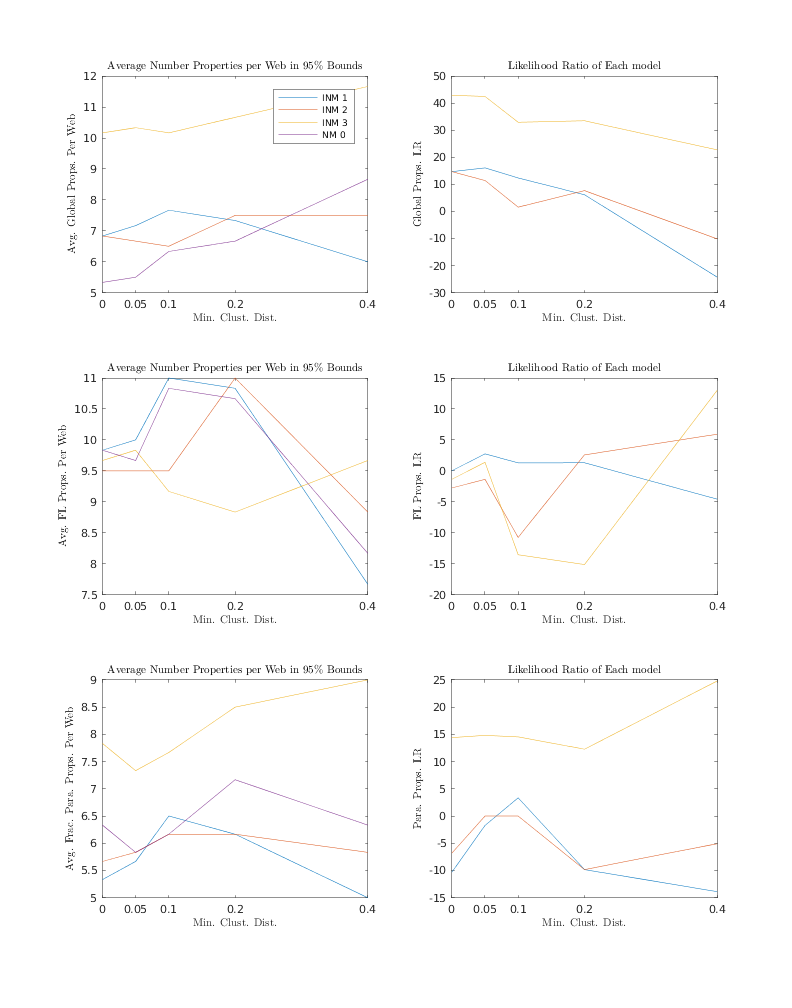
\includegraphics[width=0.8\linewidth]{\DissertationDir/Chapter3/figures/Fracs-LRs-Raw.png}
     \caption[Performance of niche models on agglomerated webs raw properties]{This figure shows the performance of each food web in terms of
         the number of properties predicted and the log-likelihood ratio,
         averaged across all empirical webs tested.
 \label{fig:ErrorsAggRaw}}
 \end{figure}

\subsection{Principal Components}

Figure \ref{fig:NMPropsPCA} provides a graphical representation of the
performance of how well the principal components of the ensemble properties
match the corresponding linear combinations of empirical web properties. We see
first that the number of principal components found within the 95\% bounds of
the ensemble data is much lower than the number of properties within the same
bounds for all webs and all models. This is expected because we are now
counting only properties that are independent of one another; some of the raw
properties tended to move together, meaning that you are likely to predict all
or none of certain subsets of the raw properties.

The subweb model still clearly predicts the most global and parasite
components. The subweb model predicts significantly more free liver properties
than the connectance and generality models and the same number of free
liver properties as the null model. The pattern of underestimation in the raw
properties is not as pronounced in the components, thus the empirical
components are about as equally likely to be over predicted as under
predicted.


\begin{sidewaysfigure}
    \centering
    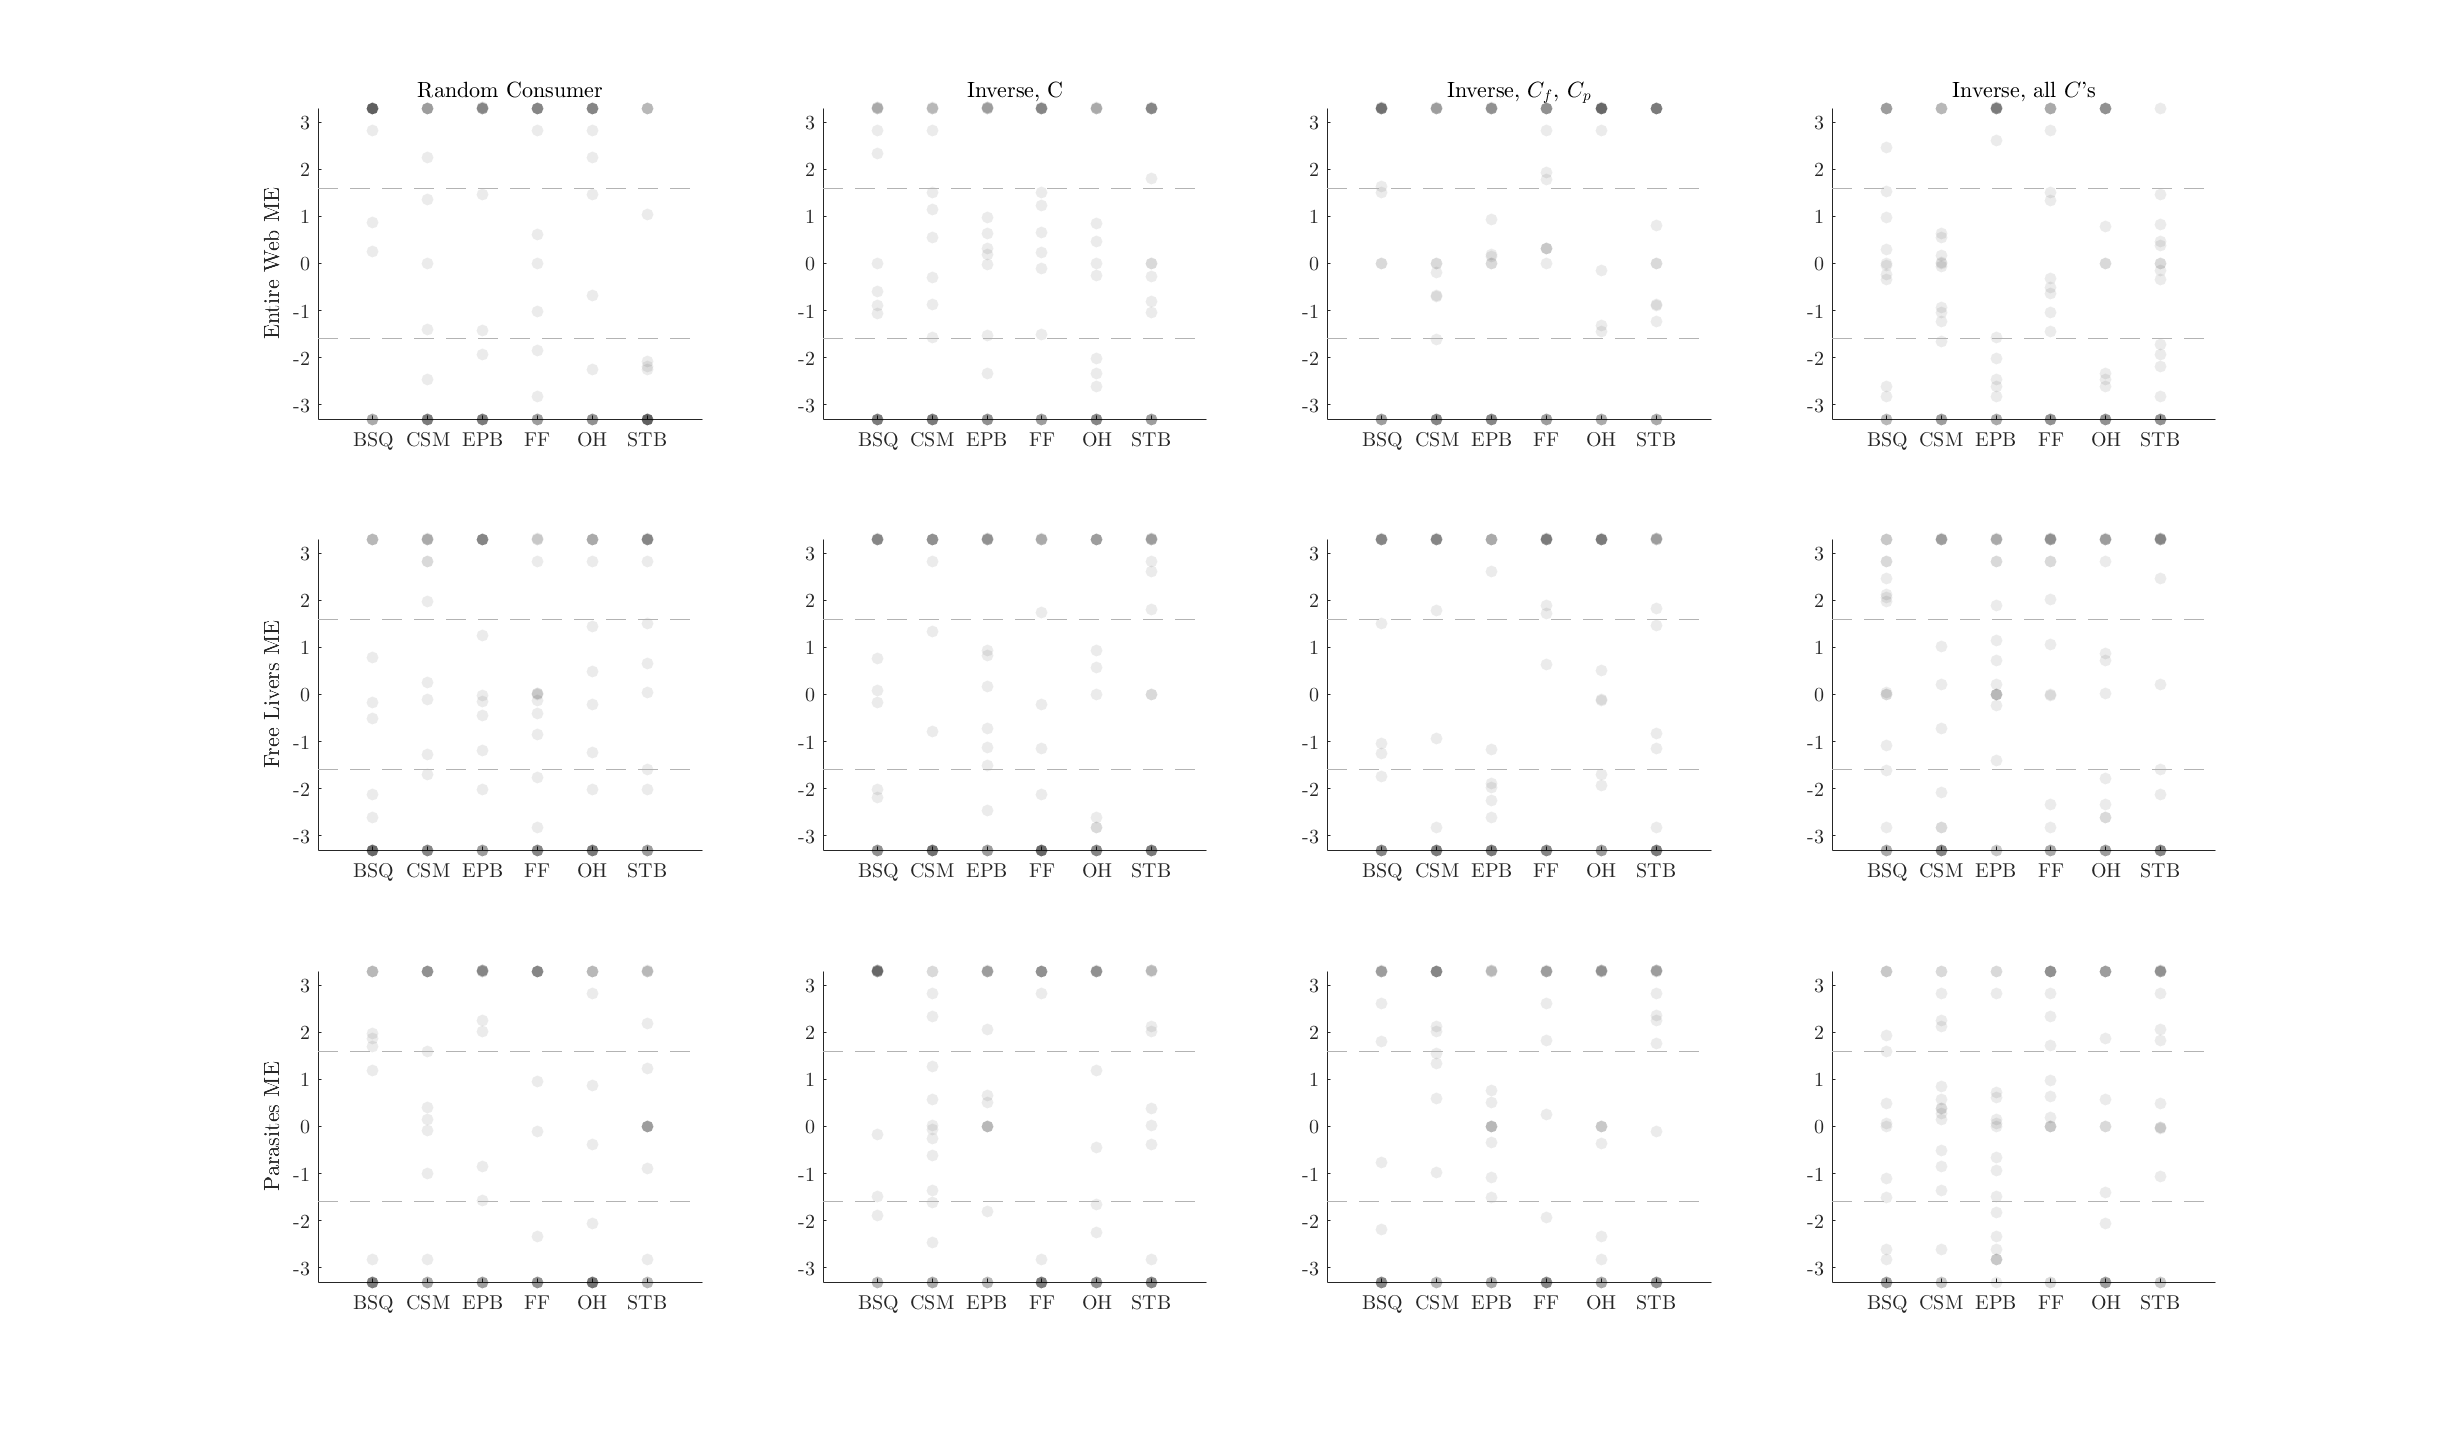
\includegraphics[width=\linewidth]{\DissertationDir/Chapter3/figures/Properties-PCA.png}
    \caption[Niche model principal components predicted]{This figure shows the percentiles of the empirical principle
        component scores. Dots represent a logit transformation of the
        percentile of each property within the ensemble.  Dots on the
        horizontal axes represent empirical property values that are completely
        outside the observed bounds of that property in the ensemble of
        simulated food webs.
    \label{fig:NMPropsPCA}}
\end{sidewaysfigure}

Figure \ref{fig:NMErrorsAggPCA} shows the performance of the four models when
predicting the principal components on the aggregated webs. When predicting
global properties (figure \ref{fig:NMErrorsAggPCA}, top row), the performance
of the subweb model declines as aggregation increases, and the other three
models are mostly unchanged. At the highest level of aggregation, the
generality model predicts significantly more components than the other three
models.

The performance of the models when predicting principal components of the
parasite community (figure \ref{fig:NMErrorsAggPCA}, bottom row) were fairly
consistent in terms of the ranking of the models. The subweb model
generally performed as well or slightly better than the other two inverse
models, and all three inverse models performed better than the null model. 
 
As with the raw properties of free livers, the principal components of the free
livers did not show a clear best model across the levels of aggregation (figure
\ref{fig:NMErrorsAggPCA}, middle row). At some levels of aggregation, inverse
models performed significantly better than the null model, and at other the
same inverse models performed worse. There was not a clear trend across
aggregation levels.

 \begin{figure}
     \centering
     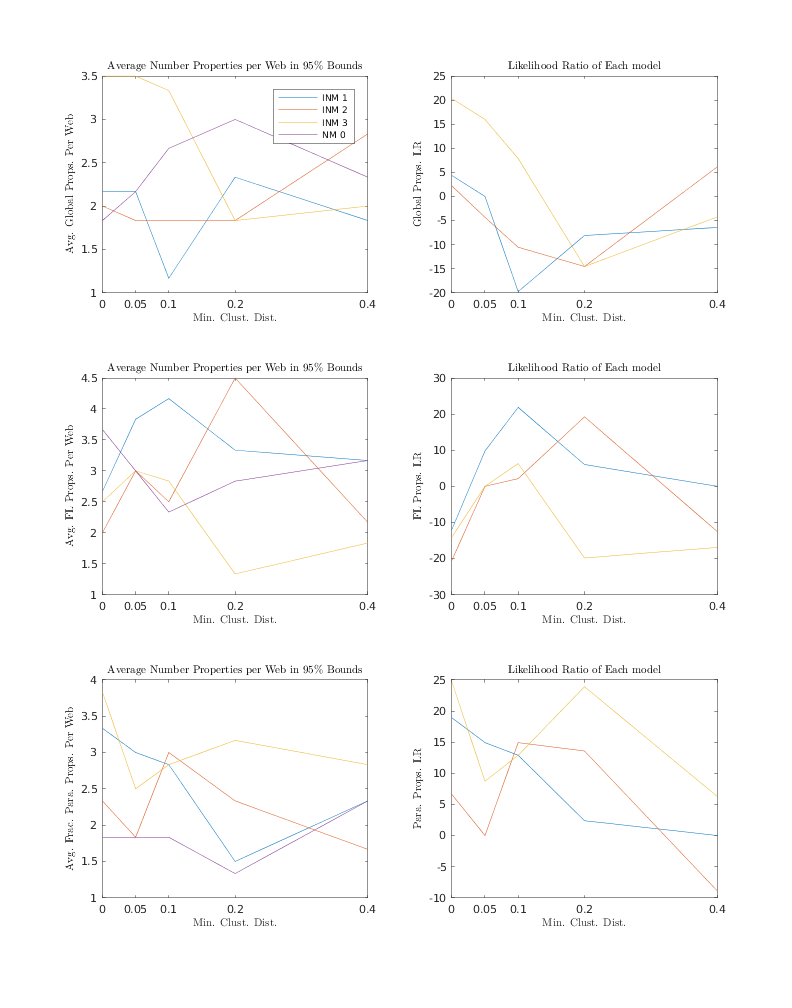
\includegraphics[width=0.8\textwidth]{\DissertationDir/Chapter3/figures/Fracs-LRs-PCA.png}
     \caption[Performance of niche models on agglomerated webs principal
     components]{This figure shows the performance of each food web in terms of
         the number of properties predicted and the log-likelihood ratio,
         averaged across all empirical webs tested.
 \label{fig:NMErrorsAggPCA}}
 \end{figure}

 
 \section{Discussion}

The subweb model performs no better than the other models on the free liver
raw properties because all four models are using the niche model to
generate free livers. It is better at predicting global properties because it
is doing better on the subwebs involving parasites. The increased performance
on the parasite subweb properties suggests that the underlying mechanisms of
smaller species eating larger species and smaller parasites being more general
than larger parasites are accurately capturing patterns in the parasite data.
\fxnote{could check the gen. of para vs. body size.} This in turn suggests that
the overall correlations between the niche axis and body size can be preserved
by making allowances for the unique body size preferences of parasitic species. 

The fact that the subweb model performs much better than the generality
model suggests that the relative frequency of the consumption of parasites is
an important feature of their structural characteristics. The subweb model
adjusts the mean diet width of free livers and parasites \textit{when they are
consuming parasites}. If the relative frequency of links with parasites as
resources is controlled, we see more properties matched. Thus, contrary to the
situation with free livers, whose properties are well predicted when model food
webs are constructed based upon their generalities, a key aspect of parasitic
structural properties seems to be not only who and how much they eat, but who
they are eaten by and how often they are eaten.

The low number of properties accurately predicted can be at least partially
explained by the fact that the six webs being modeled are quite large. The
known scale dependence of the niche model means that we should expect to see
fairly low numbers of properties matched. However, the fact that the inverse
models outperformed the null model does suggest that they are capturing key
aspects of the parasite community. 

We attempted to account for the scale dependence by decreasing trophic
resolution. We observed an increase in the number of global properties
predicted by the null model as aggregation increased. This is consistent with
what we expect to see given the scale dependence of the niche model fit. The
subweb model also predicted slightly more global properties and parasite
properties of the aggregated webs. Thus, we propose that the scale dependence
of the niche model is also present in the inverse niche model. However, lacking
small food webs with parasites makes determining the scale dependence
definitively problematic. 

We also see the sampling biases in the data as problematic to assessing the
ability of the underling mechanisms of our models. The preference of parasites
to have hosts among the invertebrates and not among the larger, higher trophic
level fish and birds, means that their diets are likely centered lower in the
niche axis. The absence of plant parasites could also fundamentally change the
properties of the parasite community in these webs and potentially alter how
the models perform.

The performance of the models as judged by the principal components of the
ensemble data show that fewer features of the ensemble data agree with the
empirical webs. At low levels of aggregation, the relative performance of the
webs remains essentially unchanged, with the subweb model predicting more
global and parasite components and comparable numbers of free liver components.
The decline in the fit of the subweb model suggests that the raw properties are
becoming more correlated with each other and thus the improved fit observed in
the raw properties can be explained by that increased correlation.

\section{Conclusion}

We found that the inverse niche model best captures features of the parasite
community when matching all subweb connectances. Matching the generality of
free livers and parasites alone was not enough. Thus, the structural
characteristics of the parasite communities in the empirical webs studied are
determined not only by who they eat, but by whom and how often they are eaten.
We proposed several supplementary procedures to assess the ability of food web
models to match empirical data but more rigorous assessments of the
alternatives is warranted.

\putbib
\end{bibunit}

\end{document}
